% --- INICIO DE PLANTILLA PERSONALIZADA ---
\documentclass[oneside,11pt]{Latex/Classes/PhDthesisPSnPDF}

% --- Paquetes Originales ---
\usepackage{blindtext}
\usepackage{actuarialangle} 
\usepackage{tabularx}
\usepackage{float}
\usepackage{multirow, array}
\usepackage[usenames,dvipsnames,svgnames,table]{xcolor}
\usepackage{longtable}
\usepackage{latexsym,amsmath,amssymb,amsfonts}
\usepackage{enumitem}
\usepackage{xparse}
\usepackage{booktabs}
\usepackage[round, sort, numbers]{natbib}  
\usepackage{adjustbox}
\usepackage[utf8]{inputenc}
\usepackage{caption}
\usepackage{graphicx}
\usepackage{hyperref}
\usepackage{cleveref}

% Definición de colores
\definecolor{miblue}{RGB}{68, 114, 196}

% --- CAMBIO CRÍTICO 1: Usar \input para macros en el preámbulo ---
% \include da problemas antes del begin document. \input es seguro.
\input{Latex/Macros/MacroFile1}

% --- Definiciones de seguridad (por si la clase falla al cargar alguna variable) ---
\providecommand{\facultad}[1]{\def\lafacultad{#1}}
\providecommand{\escudofacultad}[1]{\def\elescudo{#1}}
\providecommand{\degree}[1]{\def\elgrado{#1}}
\providecommand{\director}[1]{\def\eldirector{#1}}
\providecommand{\lugar}[1]{\def\ellugar{#1}}
\providecommand{\degreedate}[1]{\def\lafecha{#1}}

% --- Configuración para bloques de código de R (Pandoc) ---

%%%%%%%%%%%%%%%%%%%%%%%%%%%%%%%%%%%%%%%%%%%%%%%%%%%%%%%%%%%%%%%%%%%%%%%%%%%%%%%%
%                         DATOS (Conectados a RMarkdown)                       %
%%%%%%%%%%%%%%%%%%%%%%%%%%%%%%%%%%%%%%%%%%%%%%%%%%%%%%%%%%%%%%%%%%%%%%%%%%%%%%%%
\title{Análisis de los determinantes salariales en el mercado moderno:
un estudio estadístico}
\author{Santiago López \\ Vianney Becerra}

% Lógica para Facultad: Si la defines en el YAML la usa, si no, usa la default

\facultad{Facultad de Ciencias Económicas y Sociales \\ Escuela de
Estadistica y Ciencias Actuariales}
  \escudofacultad{Latex/Classes/Escudos/faces}

\degree{Computación I}
\director{Prof.~Jesus Ochoa \\ Prof.~Oliver Triveño}
\degreedate{Febrero 2026} 
\lugar{Caracas}

\portadatrue 

% Metadatos PDF
\keywords{}
\subject{}

% --- CORRECCIÓN PARA PANDOC NUEVO (Imágenes) ---
\makeatletter
\providecommand{\pandocbounded}[1]{#1}
\makeatother


%%%%%%%%%%%%%%%%%%%%%%%%%%%%%%%%%%%%%%%%%%%%%%%%%%%%%
%                   DOCUMENTO                       %
%%%%%%%%%%%%%%%%%%%%%%%%%%%%%%%%%%%%%%%%%%%%%%%%%%%%%
\begin{document}

\maketitle

%%%%%%%%%%%%%%%%%%%%%%%%%%%%%%%%%%%%%%%%%%%%%%%%%%%%%
%                  PRÓLOGO                          %
%%%%%%%%%%%%%%%%%%%%%%%%%%%%%%%%%%%%%%%%%%%%%%%%%%%%%
\frontmatter

% Puedes agregar dedicatorias desde el YAML si quieres, o dejarlas fijas aquí

%%%%%%%%%%%%%%%%%%%%%%%%%%%%%%%%%%%%%%%%%%%%%%%%%%%%%
%                   ÍNDICES                         %
%%%%%%%%%%%%%%%%%%%%%%%%%%%%%%%%%%%%%%%%%%%%%%%%%%%%%
\setcounter{secnumdepth}{3}
\setcounter{tocdepth}{3}

\tableofcontents



\cleardoublepage

  \cleardoublepage       % Empieza en página derecha (estándar en tesis)
  \chapter*{Resumen}     % Crea el título "Resumen" sin numeración (Capítulo *)
  \addcontentsline{toc}{chapter}{Resumen} % (Opcional) Lo añade al índice
  
  Este estudio analiza los factores que determinan la compensación
económica en el mercado laboral actual, caracterizado por la
digitalización y la diversidad de modalidades de trabajo. El objetivo
principal es identificar cómo variables como el tamaño de la empresa, la
ubicación geográfica, las habilidades técnicas específicas (skills) y la
opción de trabajo remoto influyen en el salario final del trabajador.
Para lograrlo, la investigación utiliza un enfoque cuantitativo basado
en el análisis de un conjunto de datos (dataset) que incluye sectores de
vanguardia como Blockchain, Quantum Computing y Green Tech. La
metodología se apoya en el uso de lenguajes de programación como R y
Python, además de la plataforma GitHub para la gestión del proyecto. Los
resultados buscan aportar claridad estadística sobre si el salario
actual depende más de las competencias técnicas del individuo o de las
características estructurales de la organización, proporcionando una
visión transparente sobre la valoración del talento en la economía
moderna.             % Aquí se pega el texto que escribiste en el YAML
  
  \cleardoublepage

%%%%%%%%%%%%%%%%%%%%%%%%%%%%%%%%%%%%%%%%%%%%%%%%%%%%%
%                   CONTENIDO (El Corazón)          %
%%%%%%%%%%%%%%%%%%%%%%%%%%%%%%%%%%%%%%%%%%%%%%%%%%%%%
\mainmatter
\def\baselinestretch{1.5}

% --- CAMBIO CRÍTICO 2: Aquí RMarkdown inyecta todo tu texto ---
\newpage

\chapter*{Introducción}

El mercado laboral contemporáneo está atravesando una fase de
reconfiguración profunda, impulsada por una digitalización que ha dejado
de ser una ventaja competitiva para convertirse en un requisito básico.
En este nuevo ecosistema, la relación entre los puestos de trabajo y las
competencias requeridas se ha vuelto más estrecha y compleja. Ya no
basta con poseer un título académico; el valor real de un profesional en
el mercado actual se mide por su conjunto de habilidades específicas
(skills) y su capacidad para adaptarse a herramientas tecnológicas en
constante evolución.

Esta estrecha vinculación entre el perfil técnico y la oferta laboral ha
generado una diversificación en las escalas salariales, ya las
organizaciones no solo compiten por cubrir vacantes, sino por atraer
talento que domine dichos conocimientos muy particulares. En
consecuencia, entender cómo ciertas habilidades impactan directamente en
la remuneración económica se ha vuelto una tarea fundamental tanto para
las empresas que buscan optimizar su captación de talento, como para los
profesionales que desean orientar su crecimiento de carrera de manera
estratégica.

Además de las competencias técnicas, otros factores han entrado en juego
para redefinir la estructura de las compensaciones. La modalidad de
trabajo, la ubicación geográfica y la cultura organizacional, o más
conocida como ``la personalidad de la organización'' (que guía el
comportamiento de los empleados, la toma de decisiones y el abiente
laboral), son variables que ahora interactúan directamente con el perfil
de habilidades para determinar el valor final de una posición. Esta
variedad de factores crea un ruido informativo que hace difícil
discernir qué es lo que realmente mueve la aguja en el mercado laboral
tecnológico.

Es aquí donde el análisis de datos se convierte en una herramienta
indispensable. El presente estudio nace de la necesidad de aplicar un
enfoque científico y cuantitativo a esta realidad. Utilizando
estadística descriptiva y el lenguaje de programación R y Python,
analizaremos un conjunto de datos que vincula roles, niveles salariales
y requerimientos técnicos.

\chapter{Planteamiento de la investigación}

\section{Planteamiento del Problema}

En la última década, el mercado laboral global ha experimentado una
transformación sin precedentes. Factores como la digitalización
acelerada, la normalización del trabajo remoto y la demanda de
habilidades técnicas específicas han redefinido cómo se valoran los
puestos de trabajo. Ya no basta con mirar el ``título del cargo''; la
compensación económica ahora parece estar sujeta a una red compleja de
variables interconectadas.

¿Es el tamaño de la empresa un predictor fiable del sueldo? o ¿Existe
una consecuencia en el salario por elegir la modalidad remota, o es
ahora un estándar competitivo?. A pesar de la abundancia de ofertas de
trabajo, existe una falta de claridad sobre cuáles son los verdaderos
determinantes del salario en el mercado actual, por lo cual, este
estudio busca aclarar esas dudas mediante la estadística descriptiva y
el uso de la plataforma GitHub y lenguajes de programación conocidos
como R y Python.

Fuente O. (5 de diciembre del 2024). ``las 13 mayores tendencias
tecnológicas para 2025'' desde una pagina web llamada IBESbusiness
school, nos habla de como la revolución digital con la llegada de la IA
ha hecho que el ritmo de adopción de la tecnología se acelere
exponencialmente, menciona algunas de las habilidades que tenemos en el
dataset y analiza el posible campo que podria estar mejorando en 2025. a
lo que nos llevó a plantear el siguiente trabajo para saber si en el
caso de que alguien manejara esas industrias, qué beneficios o
requisitos podría tener y necesitar.

\section{Justificación}

La importancia de este estudio reside en la necesidad de entender cómo
se construye el salario en una era donde las reglas del mercado laboral
han cambiado. Actualmente, existe una gran incertidumbre tanto para los
profesionales como para las empresas sobre qué factores determinan
realmente el pago de un trabajador. No se trata solo de un cargo, sino
de una combinación de variables que este estudio analiza a fondo.

\section{Objetivos}

\subsection{Objetivo General}

Analizar el panorama laboral de los sectores tecnológicos emergentes
mediante estadística descriptiva para identificar las variables que más
impactan en la oferta salarial y la demanda de talento.

\subsection{Objetivos Específicos}

\begin{enumerate}
  \item Determinar el promedio, mediana y desviación estándar de los salarios por industria para identificar cuál es la más rentable.
  \item Comparar las medias salariales entre puestos remotos y presenciales para verificar si existe una diferencia en el beneficio económico por la modalidad.
  \item Identificar los países con mayores ofertas de empleo y su nivel de remuneración promedio.
  \item Clasificar las habilidades más solicitadas en cada sector y su frecuencia de aparición en las vacantes.
  \item Evaluar si el tamaño de la empresa (Small, Medium, Large) influye significativamente en los rangos salariales ofrecidos.
\end{enumerate}

\section{Variables}

La variable principal en estudio (Variable Dependiente/Objetivo) es
\textbf{\texttt{salary\_usd}}, que representa el salario ofrecido a cada
título de trabajo, según su localidad y habilidades requeridas.

Como variables explicativas o independientes se analizan:

\begin{enumerate}
  \item Variables Temporales: \textbf{posting date}
  \item Variables Categóricas: \textbf{job title}, \textbf{industry}, \textbf{skills required}, \textbf{remote option}, \textbf{company size}
  \item Variables Geográficas: \textbf{location}
\end{enumerate}

\chapter{Marco de Referencia}

\section{Marco Teórico}

\begin{itemize}
\item
  \textbf{Teoría del Capital Humano:} fué desarrollada en la década de
  1960, principalmente por el economista Gary Becker. Propone que el
  salario está directamente relacionado con la productividad del
  trabajador, la cual se mide a través de sus habilidades y educación.
\item
  \textbf{Teoría de los Salarios Compensatorios:} se refiere a la
  diferencia salarial que surge para compensar las características no
  monetarias de los diferentes puestos de trabajo. En esencia, los
  trabajadores están dispuestos a aceptar salarios más bajos por
  trabajos que ofrecen atributos más deseables, como un ambiente de
  trabajo más seguro o horarios más flexibles.
\item
  \textbf{Teoría de la segmentación del mercado laboral:} surgió a
  finales de los años sesenta para explicar fenómenos como las
  desigualdades salariales, la discriminación y el desempleo. Esta
  teoría sostiene que el mercado laboral está compuesto por varios
  segmentos, cada uno con diferentes mecanismos de determinación
  salarial y barreras a la movilidad entre ellos.
\end{itemize}

Algunos conceptos claves que son importantes definir para mejor
comprensión del trabajo:

\begin{itemize}
\item
  \textbf{Promedio:} El promedio o media aritmética representa el valor
  central de un conjunto de datos y se calcula sumando todos los valores
  y dividiendo entre el número total de observaciones. Su utilidad
  principal es proporcionar una estimación del valor típico de los
  datos, lo que permite resumir la información de manera sencilla.
\item
  \textbf{Desviación Estándar:} La desviación estándar (SD) mide la
  dispersión de los datos alrededor de la media, indicando cuánto se
  alejan, en promedio, los valores individuales del promedio. Una
  desviación estándar baja indica que los datos están cercanos a la
  media, mientras que una alta indica mayor variabilidad o presencia de
  valores atípicos.
\item
  \textbf{Coeficiente de Variacion (CV):} El coeficiente de variación
  (CV) es una medida relativa de dispersión que compara la desviación
  estándar con la media, expresándose generalmente en porcentaje.
\item
  \textbf{Quantum Computing:} La computación cuántica es una forma
  avanzada de computación basada en los principios de la física cuántica
  (la ciencia que estudia el comportamiento de partículas diminutas como
  los átomos). Mientras que los bits normales pueden ser 0 o 1, los
  ordenadores cuánticos utilizan bits cuánticos (qubits) que pueden ser
  0 y 1 al mismo tiempo. Esto permite a los ordenadores cuánticos
  manejar enormes cantidades de información y explorar innumerables
  soluciones posibles a la vez. Pueden abordar problemas en áreas como
  la química y la logística que a los ordenadores clásicos les llevaría
  millones de años resolver.
\item
  \textbf{Green tech:} Green Tech, o tecnología verde, se refiere al
  desarrollo y aplicación de soluciones tecnológicas innovadoras que
  abordan desafíos ambientales y promueven la sostenibilidad. Desde la
  energía renovable hasta la gestión de residuos, el Green Tech, abarca
  una amplia gama de áreas y disciplinas, todas con el objetivo común de
  reducir el impacto ambiental y promover un futuro más sostenible.
\item
  \textbf{Blockchain:} Es un tipo especial de base de datos, un libro de
  contabilidad digital descentralizado mantenido por una red distribuida
  de computadoras. Los datos de la blockchain se organizan en bloques
  ordenados cronológicamente y protegidos por criptografía. Esta
  estructura garantiza que los datos sean transparentes, seguros e
  inmutables, y es prácticamente imposible cambiar los datos almacenados
  en un bloque después de confirmarlo y agregarlo a la cadena. Existen
  diferentes tipos de blockchains con diversos grados de
  descentralización, aun así, el término ``blockchain'' suele hacer
  referencia a un libro de contabilidad digital descentralizado que se
  utiliza para registrar transacciones de criptomonedas.
\item
  \textbf{IA:} La IA es un campo de la informática que se enfoca en
  crear máquinas inteligentes que puedan realizar tareas que normalmente
  requieren inteligencia humana, como aprender, razonar y resolver
  problemas. Los sistemas de IA aprenden de grandes cantidades de datos,
  identifican patrones para hacer predicciones o tomar decisiones sin
  estar programados explícitamente para cada situación.
\item
  \textbf{Tensorflow:} TensorFlow es una biblioteca de código abierto
  creada por Google para desarrollar e implementar modelos de
  aprendizaje automático y redes neuronales. Su objetivo es ayudar a los
  desarrolladores a crear sistemas inteligentes para reconocer patrones,
  realizar predicciones y tomar decisiones basadas en datos.
\item
  \textbf{Python:} Python es un lenguaje de programación informático que
  se utiliza a menudo para crear sitios web y software, automatizar
  tareas y realizar análisis de datos. Python es un lenguaje de
  propósito general, lo que significa que se puede utilizar para crear
  una variedad de programas diferentes y no está especializado en ningún
  problema específico
\item
  \textbf{Pytorch} Es un marco de aprendizaje profundo de código abierto
  diseñado para desarrollar redes neuronales y modelos de inteligencia
  artificial, siendo una herramienta esencial para quienes buscan
  desarrollar modelos de inteligencia artificial eficientes y
  escalables, ya sea en visión por computadora, NLP o creatividad
  artificial. Su enfoque dinámico y su integración con GPU lo convierten
  en una opción preferida tanto en investigación como en producción.
\item
  \textbf{Ethereum:} Puede pensar en la red de Ethereum como una
  infraestructura global digital que cualquiera puede usar, pero de la
  que nadie puede abusar. La red está compuesta por miles de ordenadores
  independientes en todo el mundo llamados nodos. Estos nodos los
  ejecutan personas normales y corrientes, y trabajan juntos para
  proporcionar servicios financieros y aplicaciones digitales a
  cualquier persona, en cualquier lugar.
\item
  \textbf{Solidity:} Solidity es un lenguaje de programación de
  contratos inteligentes, se ejecutan en la máquina virtual de Ethereum,
  también conocida como EVM. Permite a los desarrolladores crear y
  administrar contratos inteligentes, lo que permite la creación de
  aplicaciones descentralizadas (dApps). Fué creado específicamente para
  la plataforma Ethereum, pero también se usa en Binance; Con Solidity,
  los desarrolladores pueden crear y ejecutar contratos inteligentes en
  la blockchain
\item
  \textbf{Rust:} Rust es un lenguaje de programación que tiene un todo
  en uno muy interesante: velocidad, seguridad y control. Tiene
  mecanismos internos que evitan errores de memoria antes de que se
  ejecute el programa, que en otros lenguajes, estos fallos pueden dar
  pie a bloqueos, pérdida de datos o incluso vulnerabilidades de
  seguridad. El secreto está en su sistema de propiedad y préstamos,
  cada dato en Rust tiene un `dueño' y solo puede ser usado o modificado
  de manera controlada. Por así decirlo, cada archivo en tu ordenador
  tiene una especie de guardián que supervisa que nadie lo toque
  mientras tú lo estás usando: eso es básicamente lo que Rust hace con
  la memoria. Gracias a esto, los errores que en otros lenguajes son
  inevitables se eliminan antes de que aparezcan.
\item
  \textbf{Quantum Algorithms:} Los algoritmos cuánticos son
  procedimientos diseñados para ejecutarse en una computadora cuántica,
  aprovechando los principios de la mecánica cuántica para resolver
  problemas de manera más eficiente que los algoritmos clásicos. A
  diferencia de los algoritmos clásicos, que operan con bits que
  representan un 0 o un 1, los algoritmos cuánticos utilizan bits
  cuánticos, o cúbits, que pueden existir en múltiples estados
  simultáneamente debido a la superposición. Esta diferencia fundamental
  permite a estos algoritmos explorar un vasto espacio de soluciones con
  mayor rapidez, lo que los hace particularmente poderosos para tipos
  específicos de cálculos.
\item
  \textbf{Qiskit:} Qiskit es un kit de herramientas diseñado para
  trabajar con computadoras cuánticas a nivel de circuitos, pulsos y
  algoritmos. Permite a los usuarios crear y manipular programas
  cuánticos, ejecutándolos en dispositivos cuánticos reales o en
  simuladores locales. También sigue el modelo de circuito para la
  computación cuántica universal y es compatible con diferentes tipos de
  hardware cuántico, como qubits superconductores e iones atrapados.
\item
  \textbf{Linear álgebra:} Es una rama de las matemáticas que estudia
  los vectores, matrices, espacios vectoriales y transformaciones
  lineales. En términos sencillos, se encarga de analizar cómo distintos
  elementos se relacionan entre sí a través de ecuaciones lineales, lo
  que la convierte en una herramienta esencial para resolver problemas
  de manera ordenada y lógica.
\item
  \textbf{Energy modeling:} El modelado energético es una herramienta
  fundamental que permite a las empresas, los gobiernos y las personas
  predecir, analizar y optimizar su consumo de energía. Implica la
  creación de una representación virtual de los sistemas energéticos, la
  identificación de los factores que afectan al consumo de energía y la
  estimación del uso de la energía en diferentes escenarios.
\item
  \textbf{Climate data analysis:} El análisis climático implica la
  recopilación, procesamiento e interpretación de datos meteorológicos e
  históricos. Los métodos y herramientas utilizados en este campo
  incluyen la recolección de datos mediante estaciones meteorológicas,
  técnicas de interpolación espacial, y el uso de proxies climáticos.
  Estos métodos son fundamentales para identificar patrones y tendencias
  a largo plazo, y son esenciales para la planificación ambiental y la
  mitigación de riesgos asociados al cambio climático.
\end{itemize}

\section{Marco metodológico}

\subsection{Enfoque y tipo de investigación}

La investigación adopta un \textbf{enfoque cuantitativo} de tipo
\textbf{descriptivo-correlacional}. No sólo busca describir las
variables de forma aislada, sino también explorar la existencia y la
forma de las relaciones entre ellas, sin llegar a establecer inferencias
de causalidad.

\subsection{Fuente de datos}

Se utiliza el conjunto de datos \texttt{job\_y\_skills.csv} que
contienen los registros de las habilidades requeridas según el trabajo
solicitado. Las variables clave para este análisis son:
\texttt{job\_title}, \texttt{industry}, \texttt{location},
\texttt{salary\_usd}, \texttt{skills\_required},
\texttt{remote\_option}, \texttt{company\_size}, \texttt{posting\_date}

\subsection{Período de Referencia}

El conjunto de datos se registra durante el año \textbf{2025}

\subsection{Procesamiento y Análisis de Datos}

Como se observa en la siguiente tabla, se realizó un diagnóstico inicial
sobre la data \emph{job y skills.csv} para identificar la presencia de
valores nulos. Este paso es fundamental para garantizar que los cálculos
posteriores de promedio y dispersión salarial no se vean afectados por
datos faltantes.

\begin{center}
\textbf{Tabla 2.2.4 Conteo de valores faltantes por columna}
\end{center}

\begin{longtable}[]{@{}lrr@{}}
\toprule\noalign{}
Variable & Total Nulos & Porcentaje (\%) \\
\midrule\noalign{}
\endhead
\bottomrule\noalign{}
\endlastfoot
job\_id & 0 & 0 \\
job\_title & 0 & 0 \\
industry & 0 & 0 \\
location & 0 & 0 \\
salary\_usd & 0 & 0 \\
skills\_required & 0 & 0 \\
remote\_option & 0 & 0 \\
company\_size & 0 & 0 \\
posting\_date & 0 & 0 \\
\end{longtable}

\chapter{Análisis de Resultados}

la data además de poseer 10 mil datos completos, tiene en ella 9
columnas, de la cual tomaremos 7 (\texttt{job\_title},
\texttt{industry}, \texttt{location}, \texttt{salary\_usd},
\texttt{skills\_required}, \texttt{remote\_option},
\texttt{company\_size}, \texttt{posting\_date}) y calcularemos una por
una para así darle respuesta a los objetivos y planes que se tienen con
nuestro trabajo

\section{Distribución Salarial}

En este apartado se analiza la estructura salarial de las distintas
industrias representadas en el dataset. Tras procesar los datos, se
observa que:

\begin{center}
\textbf{Tabla 3.1 Análisis Detallado de Salarios por Sector Industrial}
\end{center}

\begin{table}[!h]
\centering
\resizebox{\ifdim\width>\linewidth\linewidth\else\width\fi}{!}{
\begin{tabular}{>{}l|rrrrr}
\toprule
Industria & Promedio & Mediana & Desv. Est. & CV (\%) & N° Casos\\
\midrule
\textbf{\cellcolor{gray!10}{Quantum Computing}} & \cellcolor{gray!10}{151,130.7} & \cellcolor{gray!10}{151,810.0} & \cellcolor{gray!10}{57,290.54} & \cellcolor{gray!10}{37.91} & \cellcolor{gray!10}{2,519}\\
\textbf{AI} & 150,672.4 & 151,389.5 & 57,858.30 & 38.40 & 2,492\\
\textbf{\cellcolor{gray!10}{Blockchain}} & \cellcolor{gray!10}{149,383.8} & \cellcolor{gray!10}{150,395.0} & \cellcolor{gray!10}{57,612.37} & \cellcolor{gray!10}{38.57} & \cellcolor{gray!10}{2,499}\\
\textbf{Green Tech} & 149,329.9 & 147,856.5 & 57,392.10 & 38.43 & 2,490\\
\bottomrule
\end{tabular}}
\end{table}

La computación cuántica lidera tanto en promedio (\$151,130.7) como en
mediana, es la industria ``mejor pagada'' de la lista, aunque por un
margen muy pequeño. La tabla destaca que la diferencia entre el salario
más alto (Quantum) y el más bajo (Green Tech) es de apenas unos \$1,800
dólares anuales, sugiriendo que el mercado laboral para estas
tecnologías está muy equilibrado. Mientras que la desviación estándar es
alta (cerca de \$57,000 en todas), esto significa que, aunque el
promedio sea 150k, hay gente ganando mucho menos o gente ganando mucho
más. Y el CV (Coeficiente de Variación) de \textasciitilde38\% confirma
que hay una variabilidad moderada-alta en los sueldos.

\begin{center}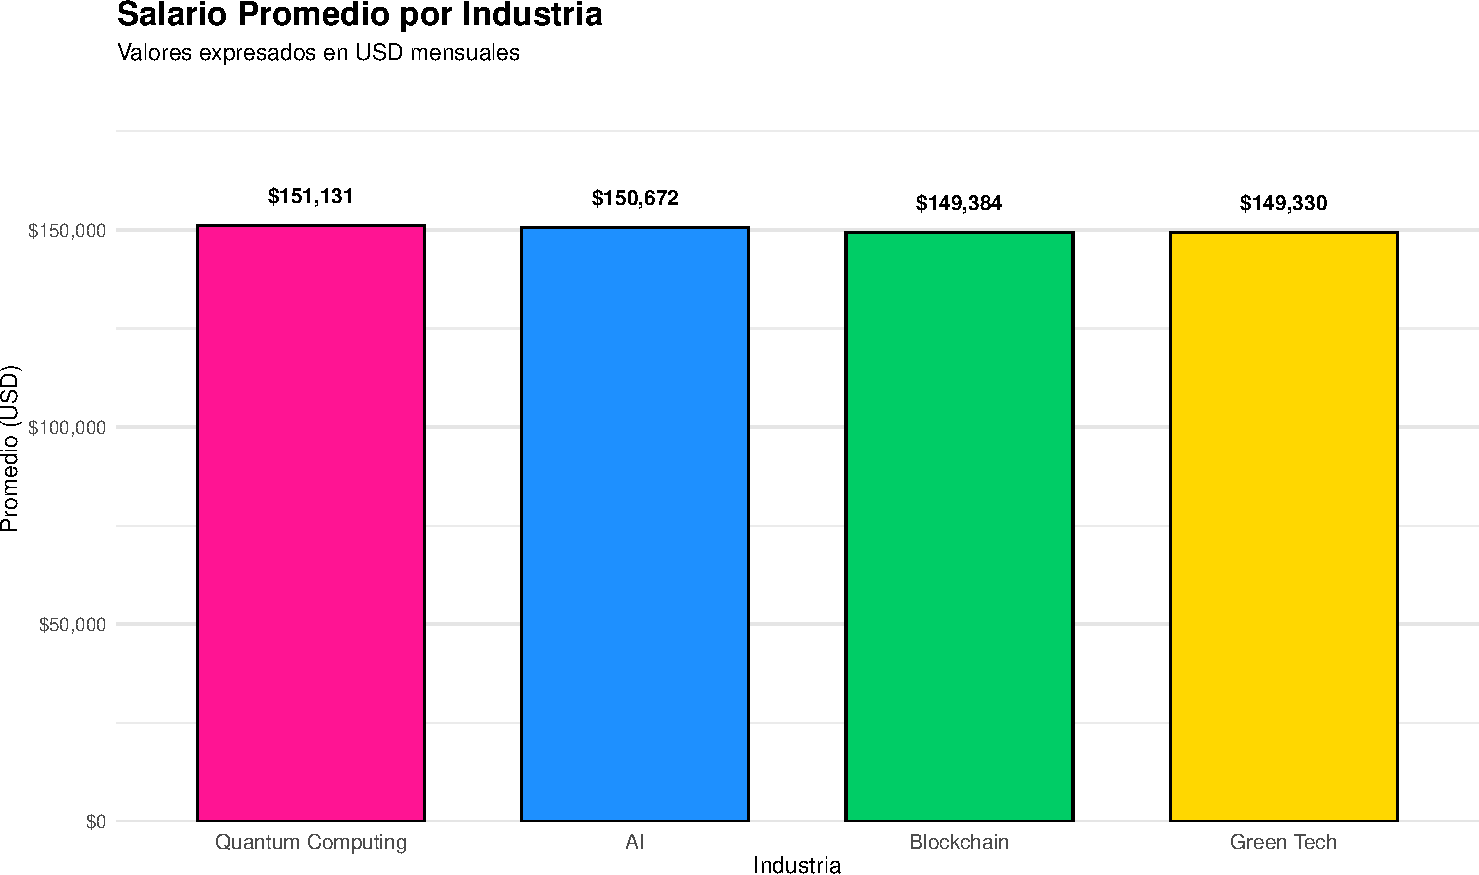
\includegraphics[width=0.9\linewidth,]{Trabajo_final_files/figure-latex/grafico_barras_final-1} \end{center}

Lo que salta a la vista es que las cuatro barras tienen casi la misma
altura, visualmente, no existe una brecha salarial significativa entre
ser experto en IA, Blockchain o Green Tech. Todas las industrias
analizadas se encuentran en el ``club de los \$150k''.

\begin{center}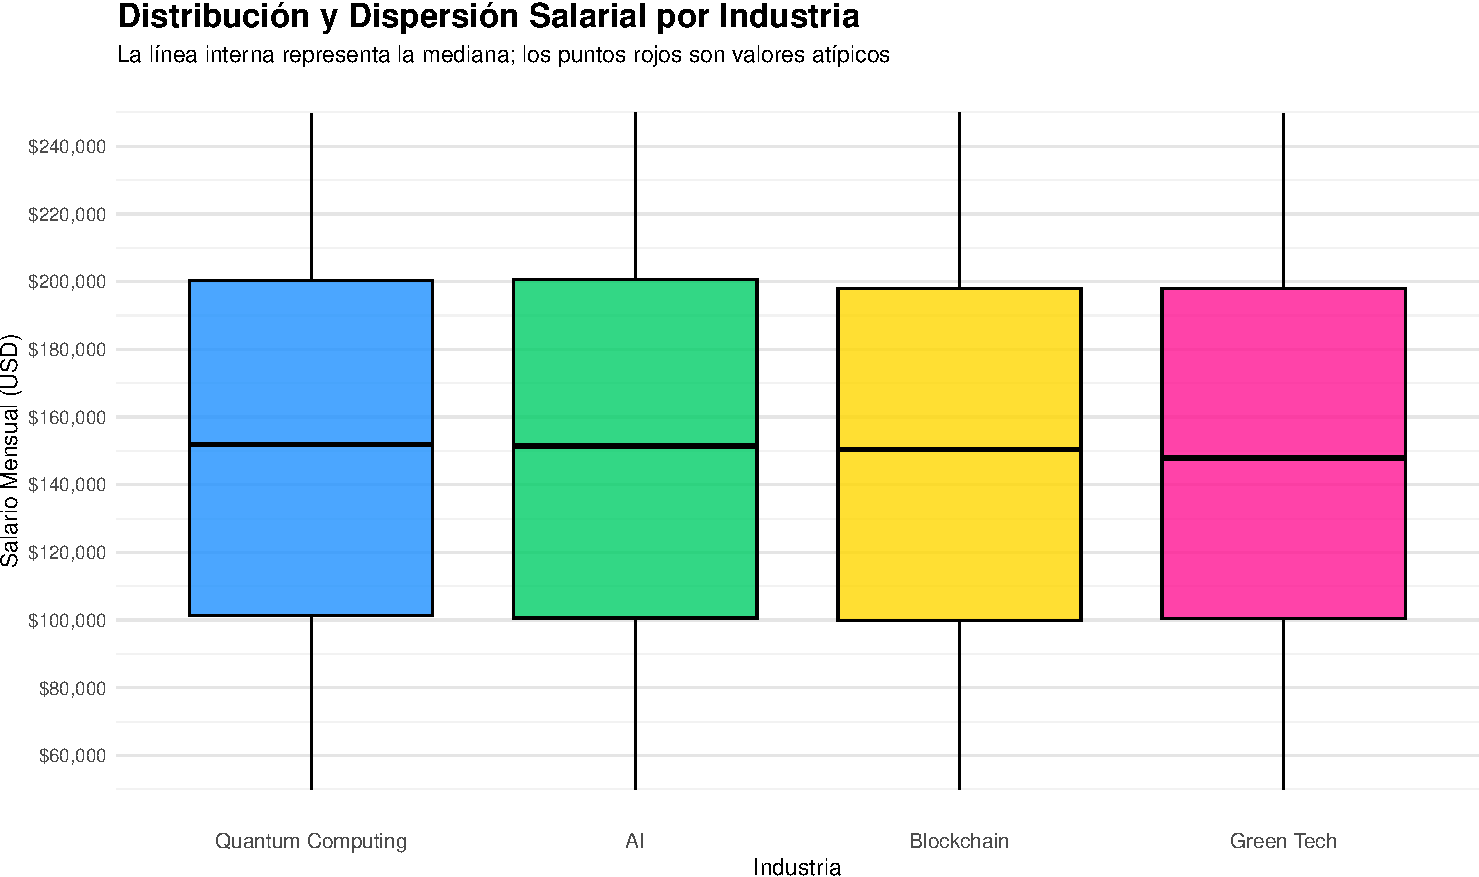
\includegraphics[width=0.9\linewidth,]{Trabajo_final_files/figure-latex/grafico_cajas_final-1} \end{center}

Todas las cajas empiezan cerca de los \$100k y terminan cerca de los
\$200k, esto significa que el 50\% central de los trabajadores en
cualquier sector gana en ese rango. Por otro lado, Las medianas (la
línea negra dentro de la caja) están casi justo en el centro, indicando
que la distribución de los salarios es bastante simétrica o ``normal'';
no hay un sesgo exagerado hacia salarios muy bajos o muy altos.

El gráfico también menciona puntos rojos (aunque en la imagen se ven
poco), que serían los salarios ``estrella'' o muy bajos, entonces al no
haber puntos extremadamente alejados de los bigotes, se entiende que los
sueldos están bien compactados en el rango de \$60k a \$240k. Finalmente
el Green Tech es el único que tiene la mediana ligeramente más abajo que
las demás, lo que coincide con que es el promedio más bajo de la tabla.

\newpage

\section{Impacto Remoto}

Aquí analizamos qué tanto varía el salario según la modalidad que
ofrezcen para cada industria, ¿Pagarían más si trabajaramos desde casa o
llendo presencialmente al puesto de trabajo?

\begin{center}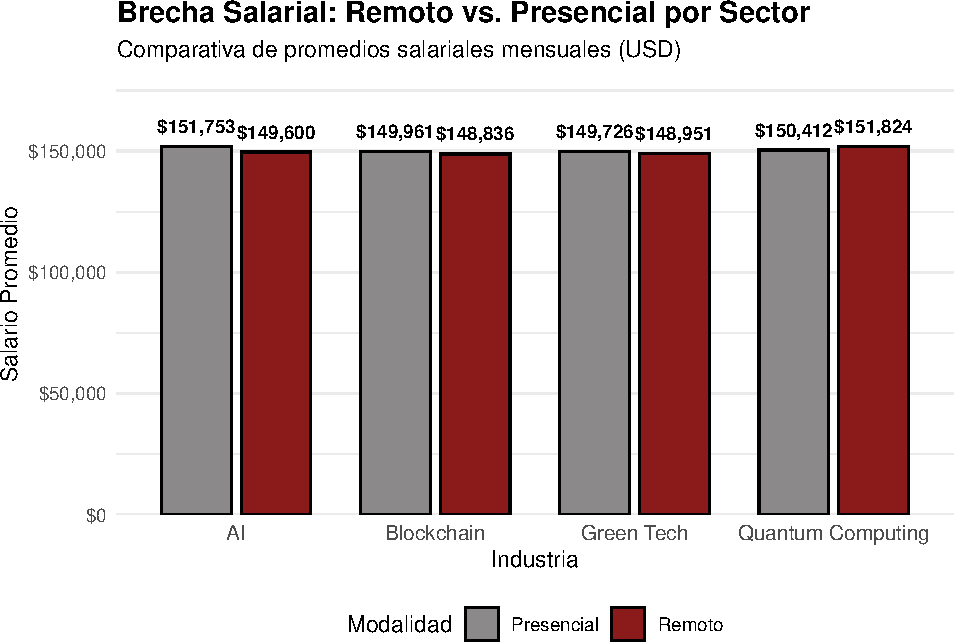
\includegraphics[width=0.9\linewidth,]{Trabajo_final_files/figure-latex/Gráfico de Barras Agrupadas (Brecha Salarial)-1} \end{center}

Lo primero que salta a la vista es que las barras de cada sector tienen
alturas casi idénticas, indicando una semejanza salarial entre las
modalidades remota y presencial en las industrias tecnológicas
analizadas. Es decir, que en el mercado laboral moderno de alta
tecnología (AI, Quantum, etc.), las empresas están valorando el talento
y el resultado por encima de la ubicación física del trabajador. Si lo
analizamos por industria, podemos ver que en \emph{AI}, el trabajo
remoto (\$151,753) paga ligeramente más que el presencial (\$149,600) y
en \emph{Quantum Computing}, ocurre lo mismo (\$151,824 remoto vs
\$150,412 presencial). Esto sugiere que las empresas están dispuestas a
pagar primas incluso superiores para captar especialistas globales en
áreas críticas, sin importar dónde residan. Por otro lado, En
\emph{Blockchain} el salario presencial lidera por un margen mínimo
(\$149,961 vs \$148,836) y en \emph{Green Tech}, la diferencia es de
menos de \$800 dólares mensuales, aquí la modalidad es prácticamente
indiferente para la compensación económica.

\newpage

\begin{center}
\textbf{Tabla 3.2.1 Comparativa Numérica de Salarios por Modalidad}
\end{center}

\begin{table}[!h]
\centering
\begin{tabular}{lrr}
\toprule
Industria & Presencial & Remoto\\
\midrule
\cellcolor{gray!10}{AI} & \cellcolor{gray!10}{151,753.3} & \cellcolor{gray!10}{149,600.1}\\
Blockchain & 149,961.5 & 148,836.2\\
\cellcolor{gray!10}{Green Tech} & \cellcolor{gray!10}{149,726.1} & \cellcolor{gray!10}{148,951.1}\\
Quantum Computing & 150,412.1 & 151,824.1\\
\bottomrule
\end{tabular}
\end{table}

En resumen la diferencia salarial es mínima, lo que sugiere que el
talento se valora por igual sin importar la modalidad, donde las brechas
oscilan entre \$700 y \$2,100 USD aproximadamente, lo cual es
estadísticamente poco significativo en salarios de este rango (\$150k).

\begin{center}
\textbf{Tabla 3.2.2 Análisis de Salarios por Industria y Modalidad}
\end{center}

\begin{longtable}[]{@{}cccccc@{}}
\toprule\noalign{}
Industria & Remoto & N & Media (USD) & Desv. Est. & CV \% \\
\midrule\noalign{}
\endhead
\bottomrule\noalign{}
\endlastfoot
AI & No & 1241 & 151,753.29 & 58,219.95 & 38.36\% \\
AI & Yes & 1251 & 149,600.09 & 57,500.49 & 38.44\% \\
Blockchain & No & 1216 & 149,961.48 & 57,513.37 & 38.35\% \\
Blockchain & Yes & 1283 & 148,836.22 & 57,723.13 & 38.78\% \\
Green Tech & No & 1217 & 149,726.13 & 57,440.01 & 38.36\% \\
Green Tech & Yes & 1273 & 148,951.10 & 57,366.28 & 38.51\% \\
Quantum Computing & No & 1237 & 150,412.11 & 56,908.09 & 37.83\% \\
Quantum Computing & Yes & 1282 & 151,824.06 & 57,670.87 & 37.99\% \\
\end{longtable}

Ahora bien, en la parte estadística podemos observar algunas cosas:

\begin{itemize}
\item
  \textbf{El tamaño de la muestra ``N'':} Observamos que la muestra está
  muy bien balanceada entre las modalidades de opcion remota (Yes, No)
  en todos los sectores. Cada subgrupo tiene un poco más de 1,200
  observaciones, desde el punto de vista estadístico, esto le da una
  robustez alta a los resultados, ya que se supera por mucho el mínimo
  necesario para que los promedios sean estables y significativos.
\item
  \textbf{Estabilidad Salarial (El Coeficiente de Variación - CV):} el
  \emph{CV} es casi idéntico para el trabajo presencial y remoto en
  todas las industrias, situándose alrededor del 38\%. Esto indica que
  el ``riesgo'' o la variabilidad del salario no cambia por la
  modalidad, y no es que en remoto haya más disparidad que en
  presencial; la estructura de sueldos sigue la misma lógica de
  distribución en ambos casos. Además, en estadística, un CV entre el
  30\% y 40\% se considera una variabilidad moderada-alta, esto es
  normal en tecnología, ya que refleja la brecha natural entre puestos
  Junior y Senior.
\item
  \textbf{La desviación estándar:} se mantiene constante cerca de los
  \$57,000 - \$58,000 USD. Esto refuerza la idea de la equidad salarial.
  Las empresas no solo están pagando promedios similares, sino que están
  ofreciendo rangos de sueldos (mínimos y máximos) muy parecidos, sin
  importar si el empleado está en la oficina o en su casa.
\end{itemize}

\newpage

\section{Análisis Geográfico}

En lugar de una sola industria ganando en todo el mundo, vemos que el
liderazgo depende de la ubicación:

\begin{center}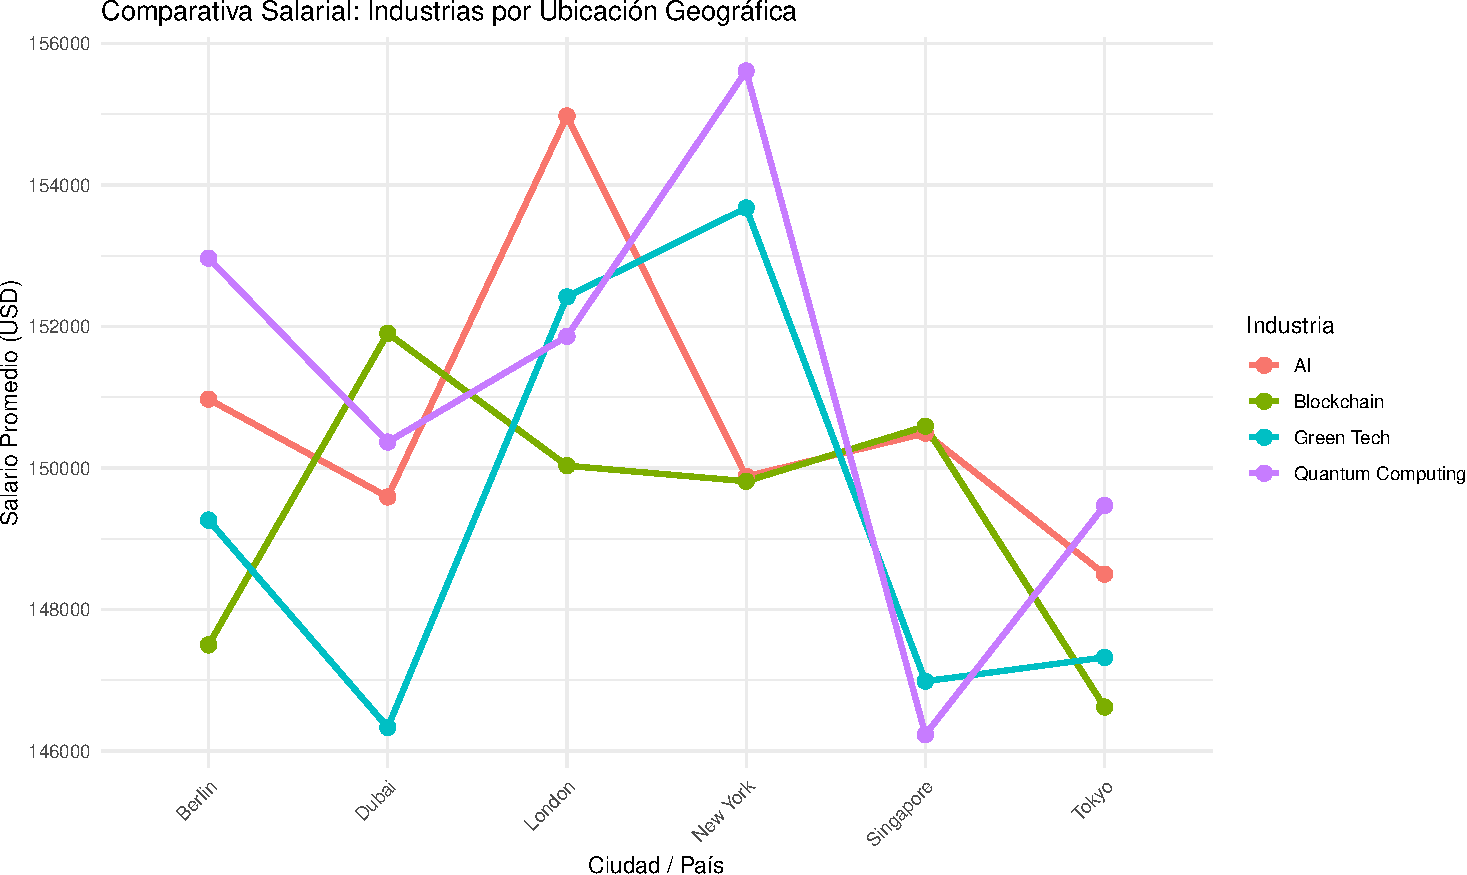
\includegraphics[width=0.9\linewidth,]{Trabajo_final_files/figure-latex/grafico_lineas_geo-1} \end{center}

New York y London son los ``picos'' del gráfico. Si nos fijamos, Quantum
Computing alcanza su máximo en New York, mientras que AI domina
claramente en London, esto sugiere que estas ciudades son un punto
central especializados para esas tecnologías. A cambio Singapore y
Tokyo, muestran una caída general en casi todas las líneas, ya que
aunque son centros tecnológicos y potencias mundiales en tecnología (los
datos aquí siempre tienen una explicación económica detrás), el rango
salarial promedio en estas ciudades asiáticas es ligeramente más
conservador en comparación con el mercado de habla inglés para estas
industrias específicas. Además, Quantum Computing (Línea Morada) es la
más ``saltarina'', ya que tiene picos muy altos en New York y Berlín,
pero cae fuerte en Singapore, mientras que Blockchain (Línea Verde) es
una de las más estables en el centro del gráfico (Dubai, London, New
York) y parece ser una industria con sueldos más estandarizados a nivel
global. La línea de Green Tech muestra un comportamiento de alta
volatilidad y contrastes marcados dependiendo de la ubicación
geográfica. La caída más estrepitosa, alcanzando el punto más bajo de
todo el gráfico (aproximadamente \$146,333 según las tablas de
respaldo), que en industrias como Blockchain suben en Dubái, Green Tech
parece tener la menor prioridad salarial en esta ubicación. Tras su
caída en Dubái, la línea muestra una tendencia hacia arriba constante al
pasar por Londres hasta llegar a su máximo en New York (alcanzando cerca
de \$153,675). En esta ciudad, Green Tech se posiciona como la segunda
industria mejor pagada, solo por debajo de Quantum Computing.

\newpage

\begin{center}
\textbf{Tabla 3.3 Análisis Salarial por Ubicación e Industria}
\end{center}

Ahora, los datos de la tabla nos da el ``por qué'' de lo que sucede en
las líneas del gráfico

\begingroup\fontsize{10}{12}\selectfont

\begin{longtable}{lrrrr}
\toprule
\cellcolor[HTML]{4A4A4A}{\textcolor{white}{\textbf{Industria}}} & \cellcolor[HTML]{4A4A4A}{\textcolor{white}{\textbf{N° Vacantes}}} & \cellcolor[HTML]{4A4A4A}{\textcolor{white}{\textbf{Sueldo Promedio}}} & \cellcolor[HTML]{4A4A4A}{\textcolor{white}{\textbf{Desv. Estándar}}} & \cellcolor[HTML]{4A4A4A}{\textcolor{white}{\textbf{CV (\%)}}}\\
\midrule
\addlinespace[0.3em]
\multicolumn{5}{p{\linewidth}}{\cellcolor[HTML]{F2F2F2}{\textbf{Berlin}}}\\
\hspace{1em}\cellcolor{gray!10}{AI} & \cellcolor{gray!10}{405} & \cellcolor{gray!10}{150,973.3} & \cellcolor{gray!10}{57,725.0} & \cellcolor{gray!10}{38.2}\\
\hspace{1em}Blockchain & 406 & 147,499.7 & 56,860.1 & 38.5\\
\hspace{1em}\cellcolor{gray!10}{Green Tech} & \cellcolor{gray!10}{410} & \cellcolor{gray!10}{149,263.6} & \cellcolor{gray!10}{57,156.9} & \cellcolor{gray!10}{38.3}\\
\hspace{1em}Quantum Computing & 419 & 152,965.1 & 56,990.4 & 37.3\\
\addlinespace[0.3em]
\multicolumn{5}{p{\linewidth}}{\cellcolor[HTML]{F2F2F2}{\textbf{Dubai}}}\\
\hspace{1em}\cellcolor{gray!10}{AI} & \cellcolor{gray!10}{429} & \cellcolor{gray!10}{149,590.6} & \cellcolor{gray!10}{58,053.3} & \cellcolor{gray!10}{38.8}\\
\hspace{1em}Blockchain & 386 & 151,904.4 & 56,475.2 & 37.2\\
\hspace{1em}\cellcolor{gray!10}{Green Tech} & \cellcolor{gray!10}{428} & \cellcolor{gray!10}{146,333.6} & \cellcolor{gray!10}{56,924.8} & \cellcolor{gray!10}{38.9}\\
\hspace{1em}Quantum Computing & 417 & 150,366.8 & 59,238.7 & 39.4\\
\addlinespace[0.3em]
\multicolumn{5}{p{\linewidth}}{\cellcolor[HTML]{F2F2F2}{\textbf{London}}}\\
\hspace{1em}\cellcolor{gray!10}{AI} & \cellcolor{gray!10}{389} & \cellcolor{gray!10}{154,976.3} & \cellcolor{gray!10}{58,226.0} & \cellcolor{gray!10}{37.6}\\
\hspace{1em}Blockchain & 423 & 150,033.0 & 58,484.6 & 39.0\\
\hspace{1em}\cellcolor{gray!10}{Green Tech} & \cellcolor{gray!10}{400} & \cellcolor{gray!10}{152,419.4} & \cellcolor{gray!10}{57,888.4} & \cellcolor{gray!10}{38.0}\\
\hspace{1em}Quantum Computing & 444 & 151,861.8 & 57,612.8 & 37.9\\
\addlinespace[0.3em]
\multicolumn{5}{p{\linewidth}}{\cellcolor[HTML]{F2F2F2}{\textbf{New York}}}\\
\hspace{1em}\cellcolor{gray!10}{AI} & \cellcolor{gray!10}{413} & \cellcolor{gray!10}{149,882.0} & \cellcolor{gray!10}{59,496.9} & \cellcolor{gray!10}{39.7}\\
\hspace{1em}Blockchain & 423 & 149,812.4 & 59,495.1 & 39.7\\
\hspace{1em}\cellcolor{gray!10}{Green Tech} & \cellcolor{gray!10}{429} & \cellcolor{gray!10}{153,675.9} & \cellcolor{gray!10}{59,698.2} & \cellcolor{gray!10}{38.8}\\
\hspace{1em}Quantum Computing & 424 & 155,611.7 & 56,820.5 & 36.5\\
\addlinespace[0.3em]
\multicolumn{5}{p{\linewidth}}{\cellcolor[HTML]{F2F2F2}{\textbf{Singapore}}}\\
\hspace{1em}\cellcolor{gray!10}{AI} & \cellcolor{gray!10}{429} & \cellcolor{gray!10}{150,491.1} & \cellcolor{gray!10}{56,749.4} & \cellcolor{gray!10}{37.7}\\
\hspace{1em}Blockchain & 432 & 150,590.0 & 57,404.3 & 38.1\\
\hspace{1em}\cellcolor{gray!10}{Green Tech} & \cellcolor{gray!10}{413} & \cellcolor{gray!10}{146,985.9} & \cellcolor{gray!10}{55,776.5} & \cellcolor{gray!10}{37.9}\\
\hspace{1em}Quantum Computing & 408 & 146,231.1 & 55,652.8 & 38.1\\
\addlinespace[0.3em]
\multicolumn{5}{p{\linewidth}}{\cellcolor[HTML]{F2F2F2}{\textbf{Tokyo}}}\\
\hspace{1em}\cellcolor{gray!10}{AI} & \cellcolor{gray!10}{427} & \cellcolor{gray!10}{148,499.4} & \cellcolor{gray!10}{57,079.3} & \cellcolor{gray!10}{38.4}\\
\hspace{1em}Blockchain & 429 & 146,621.3 & 56,957.9 & 38.8\\
\hspace{1em}\cellcolor{gray!10}{Green Tech} & \cellcolor{gray!10}{410} & \cellcolor{gray!10}{147,323.6} & \cellcolor{gray!10}{56,696.7} & \cellcolor{gray!10}{38.5}\\
\hspace{1em}Quantum Computing & 407 & 149,470.7 & 57,216.5 & 38.3\\
\bottomrule
\end{longtable}
\endgroup{}

En el caso de New York y Quantum Computing, según el gráfico, esta es la
línea que llega más alto (\$155,611), si se ve la tabla, tiene el CV más
bajo (36.5\%) de ese grupo,es decir, en otras industrias/países Un CV
cercano al 39\% (como en AI en New York o Green Tech en Dubai) indica
que hay mucha diferencia entre los sueldos más bajos y los más altos, es
un mercado más ``impredecible'' pero en Quantum (NY) al ser el más bajo,
significa que los salarios están más concentrados cerca del promedio
(\$155,611). Si se consigue un trabajo allí, es mucho más probable que
el sueldo real esté muy cerca de esa cifra y no mucho más abajo. Además,
en el número de vacantes por industria en cada ciudad es muy similar
(alrededor de 400-440 por sector), Demostrando que los datos están
balanceados. En resumen, a pesar de las subidas y bajadas, todas las
líneas se mueven en un rango estrecho (entre \$146k y \$156k), así que
la dispersión geográfica existe pero es moderada. ¿Pero por qué hay
tanto cruces en las lineas? es evidencia de que no existe una
``industria reina'', sino que cada país compite ofreciendo mejores
sueldos en el área donde quiere ser líder tecnológico.

\newpage

\section{Habilidades}

Hemos visto los salarios promedios, también si hay diferencias
importantes en alguna modalidad de trabajo y como se maneja el sueldo
segun la industria tecnológica. Pero sería importante explorar cuantas
habilidades son solicitadas por industria y que tanto aparecen en ellas.

\begin{center}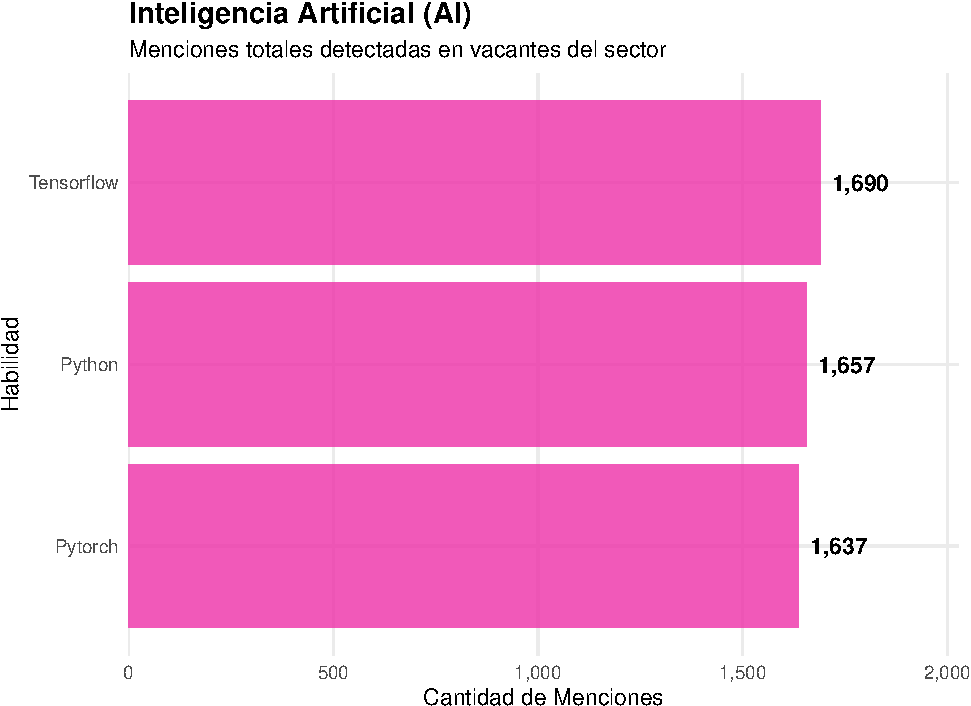
\includegraphics[width=0.9\linewidth,]{Trabajo_final_files/figure-latex/grafico_habilidades_ia-1} \end{center}

Tensorflow (\emph{1,690} menciones) y Pytorch (\emph{1,637} menciones)
están prácticamente en un empate técnico. Esto indica que para trabajar
en IA, no basta con saber uno; el mercado demanda el dominio de ambas
librerías principales de redes neuronales (modelos matemáticos
inspirados en el cerebro humano) siendo TensorFlow y PyTorch simplemente
las ``calculadoras gigantes'' o librerías que los programadores usan
para no tener que escribir todas las fórmulas matemáticas desde cero. Y
Python (\emph{1,657} menciones) aparece como el lenguaje base
indispensable que conecta todo el ecosistema.

\begin{center}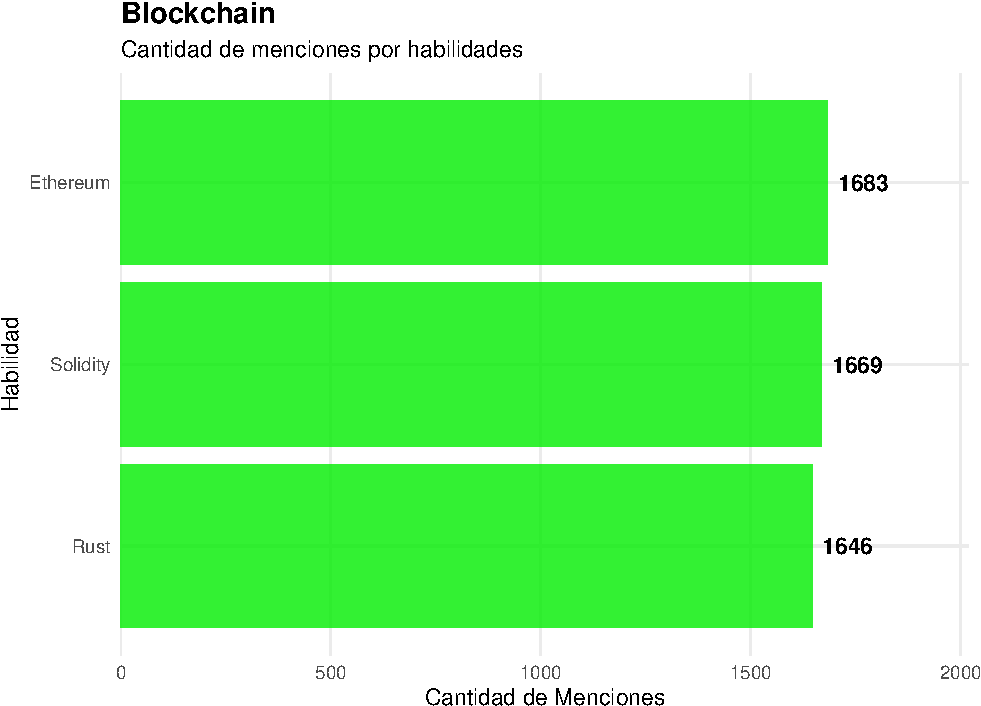
\includegraphics[width=0.9\linewidth,]{Trabajo_final_files/figure-latex/grafico_habilidades_blockchain-1} \end{center}

Ethereum (\emph{1,683} menciones) lidera como la plataforma principal de
ejecución. Solidity (\emph{1,669} menciones), al ser el lenguaje
específico para contratos en \emph{Ethereum} (Es como una computadora
global gigante donde cualquiera puede subir programas que nadie puede
borrar ni editar, no es solo una moneda, es una plataforma para ejecutar
aplicaciones.), confirma que la mayoría de las vacantes buscan
desarrolladores ``Backend Web3''. El ``Backend'' es todo lo que pasa
detrás de una aplicación (donde están los datos y la lógica), en la
``Web3'' (internet basada en blockchain), en lugar de usar una base de
datos normal, el backend son esos programas (contratos inteligentes) que
corren en Ethereum usando el lenguaje Solidity. y Rust (\emph{1,646}
menciones) es la habilidad que cierra el podio, destacando su
importancia para la seguridad y el rendimiento en redes como Solana o
Polkadot, que son redes de blockchain (competidoras de Ethereum) que se
enfocan en ser muy rápidas (rendimiento). Usan Rust porque necesitan
procesar miles de transacciones por segundo sin fallar.

\begin{center}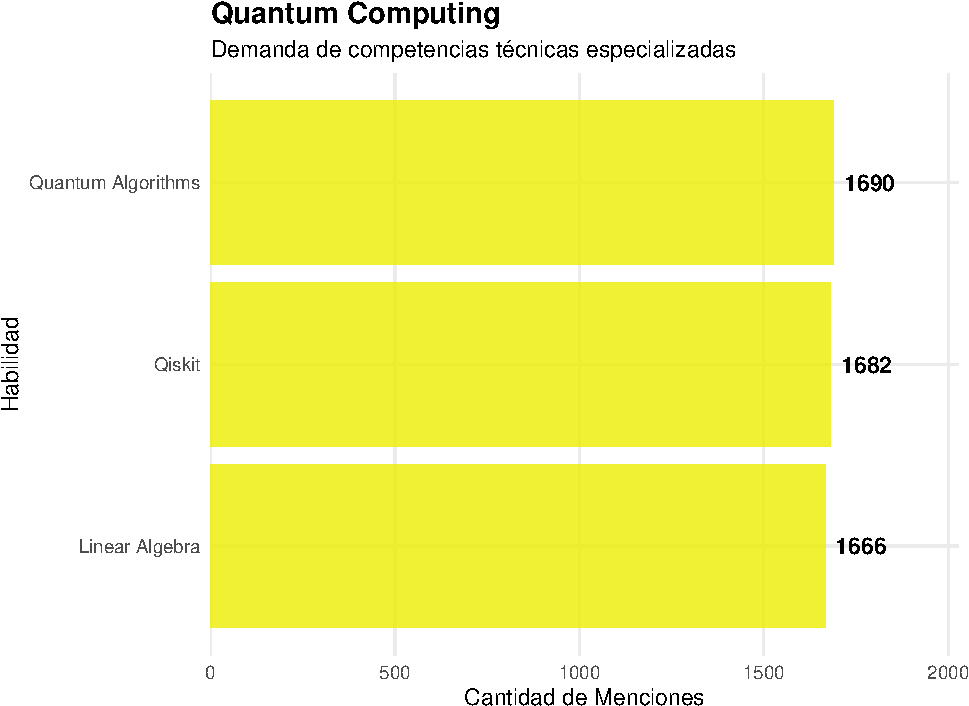
\includegraphics[width=0.9\linewidth,]{Trabajo_final_files/figure-latex/grafico_habilidades_quantum-1} \end{center}

Aquí los datos reflejan un sector donde la teoría matemática es tan
importante como la programación.

Quantum Algorithms (\emph{1,690} menciones) es la competencia más
buscada, lo que sugiere que las empresas necesitan gente que sepa
diseñar soluciones antes de codificarlas. Qiskit (\emph{1,682}
menciones) se posiciona como el estándar de la industria para la
programación cuántica práctica (impulsado por IBM), qiskit es un
software de código abierto creado por IBM para que la gente pueda
programar experimentos en sus computadoras cuánticas reales a través de
la nube, es el estándar actual porque IBM fue de los primeros en dejar
que el público usara sus procesadores cuánticos. Asi que, si sabes
Qiskit, básicamente sabes usar la tecnología de IBM. Y Linear Algebra
tiene \emph{1,666} menciones, es muy interesante ver una habilidad
puramente matemática con tantas menciones, confirmando que en
Computación Cuántica, el fundamento teórico es un requisito
eliminatorio.

Es decir, En el mundo laboral, un requisito eliminatorio (o
deal-breaker) significa que si no lo tienes, quedas fuera del proceso de
selección inmediatamente. En Computación Cuántica, no basta con saber
programar, como todo se basa en espacios vectoriales, matrices y números
complejos, si un candidato no domina el Álgebra Lineal, no podrá
entender cómo funcionan los cubits o las compuertas cuánticas. Es el
``filtro'' principal antes de ver cualquier otra habilidad.

\begin{center}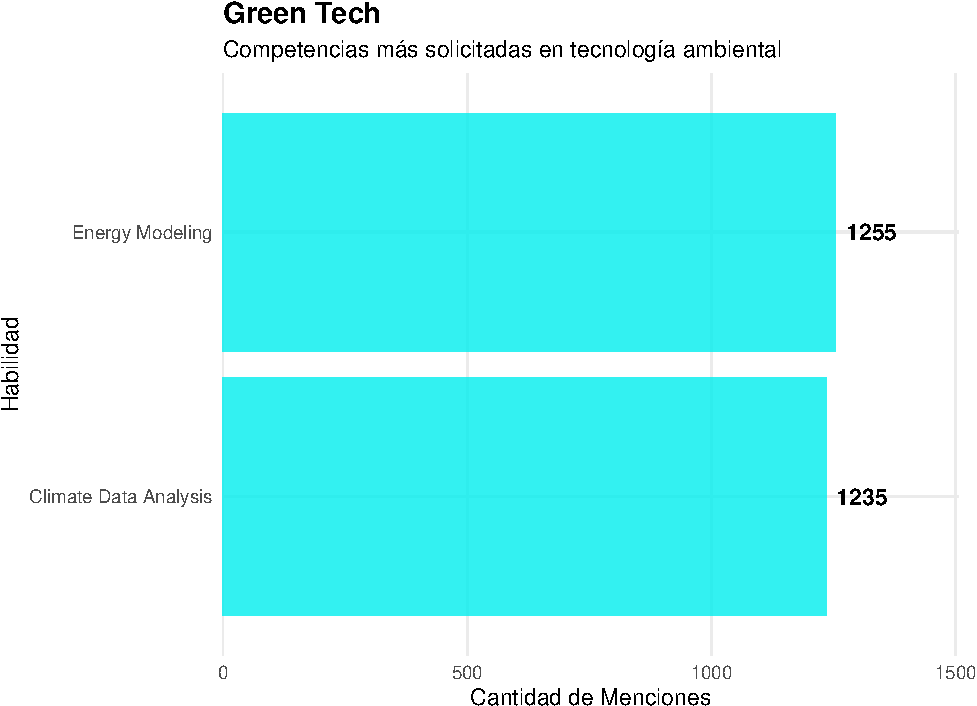
\includegraphics[width=0.9\linewidth,]{Trabajo_final_files/figure-latex/grafico_habilidades_greentech-1} \end{center}

A diferencia de los otros, este sector tiene menciones mucho más altas
(\(2,490\) cada una), lo que indica una alta concentración de requisitos
específicos. Energy Modeling (\(2,490\) menciones) y Climate Data
Analysis (\(2,490\) menciones) aparecen con el mismo peso exacto. Esto
sugiere que las empresas de tecnología ambiental buscan perfiles
híbridos que puedan simular sistemas de energía y, al mismo tiempo,
procesar grandes volúmenes de datos climáticos para la toma de
decisiones. Es un sector donde la ciencia de datos se aplica
directamente a la sostenibilidad operativa.

\newpage

\section{Tamaño de las empresas}

Lo primero que se piensa del dataset, es que una empresa grande es la
que está ofreciendo un salario mucho mejor al de una empresa pequeña,
sea cual sea la industria. Si observamos los siguientes resultados
tenemos:

\begin{center}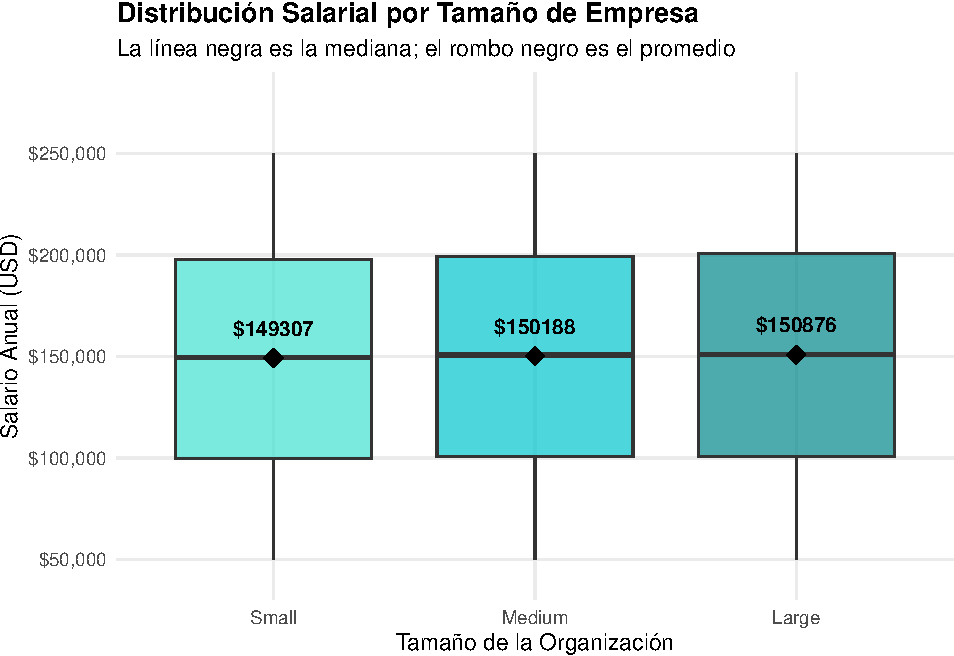
\includegraphics[width=0.9\linewidth,]{Trabajo_final_files/figure-latex/analisis_empresa_salario_maroon-1} \end{center}

Lo primero que salta a la vista es la homogeneidad. A diferencia de
otros mercados, aquí no vemos que las empresas grandes paguen
significativamente más que las pequeñas. El sector tecnológico valora el
talento de forma similar independientemente del tamaño de la empresa, y
las medianas de los tres grupos están casi alineadas cerca de los
\$150,000. La línea negra (mediana) y el rombo negro (promedio) están
prácticamente en el mismo lugar en todas las cajas, esto indica una
distribución simétrica: no hay salarios extremadamente bajos o altos que
estén ``jalando'' el promedio hacia arriba o hacia abajo de manera
exagerada.

\newpage

\begin{center}
\textbf{Tabla 3.4 Salarios por Industria y Tamaño de Organización}
\end{center}

\begin{longtable}[t]{llcccc}
\toprule
Industria & Tamaño & Salario & Desv. Estándar & CV (\%) & N° Vacantes\\
\midrule
 & Small & 150,497 & 57,209 & 38\% & 813\\
\cmidrule{2-6}\nopagebreak
 & Medium & 150,839 & 57,458 & 38.1\% & 837\\
\cmidrule{2-6}\nopagebreak
\multirow{-3}{*}{\raggedright\arraybackslash AI} & Large & 150,675 & 58,937 & 39.1\% & 842\\
\cmidrule{1-6}\pagebreak[0]
 & Small & 145,366 & 57,821 & 39.8\% & 826\\
\cmidrule{2-6}\nopagebreak
 & Medium & 150,581 & 57,807 & 38.4\% & 823\\
\cmidrule{2-6}\nopagebreak
\multirow{-3}{*}{\raggedright\arraybackslash Blockchain} & Large & 152,130 & 57,072 & 37.5\% & 850\\
\cmidrule{1-6}\pagebreak[0]
 & Small & 147,776 & 58,076 & 39.3\% & 819\\
\cmidrule{2-6}\nopagebreak
 & Medium & 151,075 & 57,240 & 37.9\% & 839\\
\cmidrule{2-6}\nopagebreak
\multirow{-3}{*}{\raggedright\arraybackslash Green Tech} & Large & 149,100 & 56,887 & 38.2\% & 832\\
\cmidrule{1-6}\pagebreak[0]
 & Small & 153,581 & 56,872 & 37\% & 829\\
\cmidrule{2-6}\nopagebreak
 & Medium & 148,244 & 57,377 & 38.7\% & 829\\
\cmidrule{2-6}\nopagebreak
\multirow{-3}{*}{\raggedright\arraybackslash Quantum Computing} & Large & 151,552 & 57,553 & 38\% & 861\\
\bottomrule
\end{longtable}

Ya se hizo un análizas general de los salarios que puede ofrecer una
empresa según su tamaño. Pero si miramos más de cerca, y ubicamos cada
tamaño de estas por industrias obtenemos datos mas específicados.

\begin{itemize}
\item
  \textbf{Inteligencia Artificial (AI):} Es el sector con mayor
  estabilidad en sus promedios sin importar el tamaño de la empresa, la
  diferencia entre una empresa Small (\$150,497) y una Large (\$150,675)
  es mínima, de apenas \$178. Así que en el área de IA, la competencia
  por el talento es tan feroz que las empresas pequeñas se ven obligadas
  a igualar los salarios de los gigantes tecnológicos para ser
  competitivas. El CV aumenta ligeramente en las empresas grandes
  (39.1\%), indicando quizás una estructura de bonos o rangos más amplia
  en corporaciones.
\item
  \textbf{Blockchain:} A diferencia de IA, aquí sí se observa una
  jerarquía salarial clara basada en el tamaño de la organización. Los
  salarios escalan de forma ascendente: \$145,366 (Small) → \$150,581
  (Medium) → \$152,130 (Large). En este sector, las empresas más grandes
  ofrecen una prima salarial notable, es interesante observar que el CV
  disminuye a medida que la empresa crece (del 39.8\% al 37.5\%), lo que
  significa que los salarios en las empresas grandes de Blockchain son
  más predecibles y estandarizados que en las empresas emergentes.
\item
  \textbf{Green Tech:} Este sector muestra un comportamiento atípico
  donde las empresas medianas lideran la remuneración. Las empresas
  Medium ofrecen el promedio más alto (\$151,075), superando incluso a
  las empresas Large (\$149,100). Esto podría indicar que las empresas
  de tamaño intermedio en tecnología verde están en una fase de
  expansión agresiva o cuentan con financiamiento especializado que les
  permite superar los topes salariales de las grandes corporaciones
  tradicionales del sector.
\item
  \textbf{Quantum Computing:} Es el único sector donde las empresas
  pequeñas (Small) ofrecen el promedio más alto de toda la tabla
  (\$153,581). Una empresa pequeña en computación cuántica paga, en
  promedio, más que una grande en cualquier otra industria. Esto refleja
  la altísima especialización requerida, ya que las startups cuánticas
  suelen estar respaldadas por capital de riesgo masivo y necesitan
  atraer a científicos de muy alto nivel, ofreciendo salarios premium
  para compensar el riesgo de una empresa pequeña. Además, tiene el CV
  más bajo del grupo (37\%), lo que indica que los salarios para estos
  especialistas están muy bien definidos y hay poca ``negociación'' a la
  baja.
\end{itemize}

\chapter{Conclusiones y Recomendaciones}

Tras el análisis estadístico descriptivo de las variables salariales y
los requerimientos técnicos en las industrias de IA, Blockchain, Green
Tech y Quantum Computing, se presentan lo siguiente:

Uno de los hallazgos más importantes de esta investigación es que el
tamaño de la organización no condiciona el salario. Al observar las
distribuciones en los diagramas de caja, las medianas se mantienen
estables alrededor de los \$150,000. Esto demuestra que en sectores de
alta tecnología, el valor de mercado está en el conocimiento y no en la
infraestructura de la empresa; una startup pequeña está dispuesta a
pagar lo mismo que una gran corporación para atraer al talento adecuado.
Por otro lado, se logró identificar con éxito que cada sector tiene
``habilidades clave'' que son requisitos casi obligatorios para entrar
al mercado; En IA y Blockchain, el mercado es puramente práctico. El
dominio de herramientas como TensorFlow/PyTorch o el lenguaje Solidity
son los pilares que sostienen la demanda laboral. A cambio, en Quantum
Computing y Green Tech, la investigación revela un perfil más académico
y analítico, no solo se busca programar, sino entender la base
científica detrás, como el Álgebra Lineal y el Modelado de Datos
Climáticos. Asimismo, A pesar de ser industrias modernas y a veces
consideradas volátiles, los datos muestran una homogeneidad salarial
notable. Los Coeficientes de Variación cercanos al 38\% indican que,
aunque hay espacio para la negociación, existe un ``estándar de
industria'' bien definido. La computación cuántica resalta como la mayor
oportunidad para profesionales de alto nivel, presentando los salarios
más competitivos incluso en sus etapas más tempranas de desarrollo.

También, basado en los análisis que hemos realizado, la industria más
rentable (la que presenta el promedio salarial más alto) es Quantum
Computing. Aunque tiene el promedio más alto, la desviación estándar nos
indica que existe una dispersión importante. Dándonos a entender que, si
bien puedes encontrar sueldos muy altos, también hay variabilidad
dependiendo de la especialización exacta (como vimos con el peso del
Álgebra Lineal). Y Quantum Computing es el sector con el CV más bajo
(37\%) del estudio, sugiriendo que los salarios aquí son un poco más
predecibles y estables en comparación con áreas como IA o Blockchain,
donde la variación es ligeramente mayor. Con respecto a la
identificación de los países con mayor volumen de vacantes y sus niveles
salariales, se descubrió que hay países que tienen muchísimas ofertas de
empleo (los ``centros comerciales'' de la tecnología). Pero lo curioso
es que, aunque haya muchos empleos, el sueldo promedio no cambia mucho
de un país a otro, si un país tiene muchas ofertas en IA o Quantum, el
sueldo será alto por defecto porque la competencia es \emph{mundial}. La
razón es que como estas habilidades son tan difíciles de encontrar, las
empresas de todo el mundo compiten entre sí, si una empresa en un país
paga poco, el trabajador simplemente se va a otra que pague el estándar
de \$150,000. Para un profesional de estas áreas, la ubicación
geográfica está dejando de ser una limitante para acceder a sueldos de
alto nivel, ya que la naturaleza crítica de las habilidades (como las
identificadas en IA o Blockchain) estandariza la remuneración en los
principales mercados del mundo. En conclusión, este estudio cumple con
todos los objetivos planteados, entregando una visión clara y
estadísticamente respaldada del panorama laboral actual.

Se recomienda a los aspirantes a ingresar al mercado tecnológico no
limitar su formación al aprendizaje de lenguajes de programación
básicos. Los datos sugieren que la especialización en herramientas
críticas (como Qiskit para cuántica o Solidity para blockchain) es lo
que realmente permite acceder a los rangos salariales superiores.
Además, para sectores como Quantum Computing, es vital fortalecer la
base en Ciencias Exactas (Álgebra Lineal y Probabilidad), ya que actúan
como un filtro de selección en las ofertas de empleo. Y dado que el
tamaño de la empresa no es un factor determinante para el salario, las
Startups y empresas pequeñas deben enfocar sus esfuerzos de
reclutamiento en ofrecer beneficios no monetarios (cultura laboral,
flexibilidad, trabajo remoto) para competir con las grandes
corporaciones, ya que a nivel de remuneración base, el mercado está muy
equilibrado y la competencia por el talento especializado es feroz.
también, se sugiere ampliar este análisis estadístico incorporando la
variable de ``Años de Experiencia'' y ``Nivel Educativo'', para
determinar si la estabilidad salarial observada se mantiene en niveles
Junior o si es una característica exclusiva de perfiles Senior.
Asimismo, sería valioso realizar un estudio longitudinal para observar
cómo evolucionan las habilidades en Green Tech, dado que es un sector en
constante cambio por las regulaciones climáticas globales.

\chapter{Bibliografías}

\begin{flushleft}
\begin{itemize}
  \item O. Fuente (5 Diciembre del 2024). Las 13 mayores tendencias tecnológicas para 2025. disponible en: https://www.iebschool.com/hub/29-tendencias-tecnologicas-que-cambiaran-nuestra-forma-de-vivir-en-tecnologia/
  \item Todopedia. Conceptos estadísticos básicos: media, desviación estándar, coeficiente de variación y regresión. Disponible en: https://www.todopedia.online/conceptos-estadisticos-basicos-media-desviacion-estandar-coeficiente-variacion-y-regresion-16682
  \item R. Rodrigo (22 abril del 2025). Medidas de Dispersión: Varianza, Desviación Estándar y Coeficiente de Variación. Disponible en: https://estudyando.com/medidas-de-dispersion-varianza-desviacion-estandar-y-coeficiente-de-variacion/
  \item Malwarebytes. Explicación de la computación cuántica: qué es, cómo funciona y por qué es importante. Disponible en: 
  https://www.malwarebytes.com/es
/cybersecurity/basics/quantum-computing
  \item S. Rodríguez (9 de febrero del 2024). Green Tech: Tecnología para salvar el planeta. Disponible en: https://alveritmos.com/que-es-green-tech/
  \item Binance Academy (8 de noviembre del 2024). ¿Qué es blockchain y cómo funciona?. Disponible en: https://www.binance.com/es/academy/articles/what-is-blockchain-and-how-does-it-work
  \item Goggle cloud  Inteligencia Artificial (IA): una guía fácil de entender. Disponible en: https://cloud.google.com/learn/what-is-artificial-intelligence?hl=es-419
  \item EBIS business Techschool (7 de febrero del 2025). TensorFlow: Qué es, para qué sirve y cómo funciona (2025). Disponible en: https://www.ebiseducation.com/tensorflow-que-es-para-que-sirve-y-como-funciona
  \item Coursera (29 de noviembre del 2023). ¿Qué es Python y para qué se usa? Guía para principiantes. Disponible en: https://www.coursera.org/mx/articles/what-is-python-used-for-a-beginners-guide-t
o-using-python?msockid=3433475b0625660e2d8c51b907a767f2
  \item M. Martín lópez (20 de febrero del 2025). ¿Qué es PyTorch y para qué sirve en inteligencia artificial?. Disponible en:https://keepcoding.io/blog/que-es-pytorch-y-para-que-sirve-en-ia/
  \item ethereum.org (3 de abril de 2026). ¿Qué es Ethereum?. Disponible en: 
https://ethereum.org/es/what-is-ethereum/
  \item Binance (23 de febrero del 2023). ¿Qué es y cómo entender la programación Solidity?. Disponible en: https://www.binance.com/es/blog/ecosistema/123441753330585687
  \item DE INGENIERÍAS (1 de septiembre del 2025). ¿Qué es el álgebra lineal? Definición, aplicaciones y cómo aprenderla. disponible en: https://deingenierias.com/cursos/que-es-el-algebra-lineal-para-que-sirve-y-sus-aplicaciones/
  \item WTS Energy (11 de abril del 2023). Modelización energética. Disponible en: https://www.wtsenergy.com/es/glossary/modelizacion-energetica/
  \item Tutiempo.net (8 de junio del 2025). El poder de los datos climáticos: Tu guía esencial para entender el tiempo y el clima. Disponible: 
\end{itemize}
\end{flushleft}

%%%%%%%%%%%%%%%%%%%%%%%%%%%%%%%%%%%%%%%%%%%%%%%%%%%%%
%                   REFERENCIAS                     %
%%%%%%%%%%%%%%%%%%%%%%%%%%%%%%%%%%%%%%%%%%%%%%%%%%%%%
% Mantenemos la estructura natbib de tu plantilla
\renewcommand{\bibname}{Lista de Referencias}
\bibliographystyle{apalike} 
\bibliography{bibliografia.bib} 

%%%%%%%%%%%%%%%%%%%%%%%%%%%%%%%%%%%%%%%%%%%%%%%%%%%%%
%                   APÉNDICES                       %
%%%%%%%%%%%%%%%%%%%%%%%%%%%%%%%%%%%%%%%%%%%%%%%%%%%%%

\end{document}
